%\section{Demonstration}
% how to evaluate?

% random picking relation, labeling true or false?
% the count precision@x?

% check: 1. GY's paper
%        2. ritter's paper

% Check their page size
% write about our size.
% and compare the version of MI-Equal, MI-Uniform, TfIdf-Equal, TfIdf-Uniform
%%In the demonstration part, we first introduce the experimental setup.
%%Secondly we evaluate the accuracy of relation type inferring.
%%Then we present our web interface of RvSp system, and finally
%%we provide some example relations with the inferred argument types.

\section{Evaluation}
% Add Freebase dump citation
%\KZ{First, say a bit about the ReVerb dataset, and the specifics of
%Freebase. Then say something about our implementation details in the
%3 steps, such as parser we used, etc. What about the numbers in the table?}


Freebase \cite{bollacker2008freebase} is a collaboratively generated knowledge base,
which contains more than 40 million entities, and more than 1,700 real types
\footnote{Freebase types are identified by type id, for example, $sports.pro\_athlete$ stands for ``professional athlete''.}.
In our experiment, We use the 16 Feb. 2014 dump of Freebase as the knowledge
base.

ReVerb \cite{fader2011identifying} is an Open IE system
which aims to extract verb based relation instances from web corpora.
The release ReVerb dataset contains more than 14 millions of relation tuples with high quality.
%Each entity belongs to at least one type.
%When compared with other knowledge bases, Freebase has a much greater focus on named entities than {\tt WordNet}.
%Besides, the type hierarchy of {\tt Yago} is too fine-grained, which is not suitable for schema inferring.
%Considering aspects mentioned above, we adapt Freebase as our knowledge base in our work.
%The input ReVerb dataset is released by Lin et al.\shortcite{lin2012entity}, containing 3 millions of relation tuples with high quality.
We observed that in ReVerb, some argument is unlikely to be an entity in Freebase, for example:

$\langle Metro\ Manila,\ consists\ of,\ \textbf{12 cities}\rangle$,

\noindent
where the object argument is not an entity but a type. Since types are usually represented by lowercase common words,
we remove the tuple if one argument is lowercase, or if it is made up
completely of common words in WordNet.
In addition, because date/time such as ``Jan. 16th, 1981''
often occurs in the object argument while Freebase does not have any
such specific dates as entities,
we use SUTime \cite{chang2012sutime} to recognize dates as an virtual entity.
After cleaning, the system collects 3,234,208 tuples and
171,168 relation groups.

% Talk about entity linking.
%We make the following parameter settings by empirics:
The following parameters are tuned using a development set:
$\tau = 0.667$,
$\epsilon=0.6$, $\lambda = 5\%$ and $\rho = e^{-50}$.
For relation grouping, we use Stanford Parser \cite{klein2003accurate}
to perform POS tagging, lemmatizing and parsing on relations.
%1. data come from Rv 3M
%2. Freebase.
% set tau to be 0.667 as the empirical value
%2. lowercased are removed
%3. remaining xxx relations, and xxx tuples.
% Important part, how to evaluate ?
%All the data sets involved in the evaluation are available at
%\url{http://202.120.38.146/schema/}.


We first evaluate the results of entity linking.
We randomly pick 200 relation instances from ReVerb, and manually
labeled arguments with Freebase entities.
For both naive and ensemble strategy, we evaluate the precision, recall, F1 and MRR score on the labeled set.
An output entity pair is correct, if and only if both arguments
are correctly linked. Experimental results are listed in \tabref{tab:linking_result}.

%We assigned 3 human annotators to judge whether both arguments are linked to correct entities.
%We don't have a gold set for entity linking, but we assume that each unlinked relation tuple corresponds to a linked tuple.
%Therefore, we can approximate the recall of entity linking as:
%\begin{equation}
%recall\ =\ \frac {precision * \#Linked\ Tuples} {\#Relation\ Tuples}
%\end{equation}
%For each strategy, the total number of linked tuples, precision, recall and F1 are listed in \tabref{tab:linking_result}.

\begin{table}[ht]
\small
	\centering
	\caption{Entity Linking Result}
	\begin{tabular}{Ic|c|c|c|cI}
		%\toprule
        \whline
		Strategy & P & R & F1 & MRR \\
        \whline
        Naive    & 0.371 & 0.327 & 0.348 & 0.377 \\
        \hline
        Ensemble & 0.386 & 0.340 & 0.361 & 0.381 \\
        \whline
	\end{tabular}%
	\label{tab:linking_result}%
\end{table}

For the evaluation of relation schema, we first randomly pick
50 binary relations with support larger than 500 from the system.
For each relation, we selected top 100 type pairs with the largest
support, as what we evaluated.
We assigned 3 human annotators to label the fitness score of type
pair for the relation. The labeled score ranges from 0 to 3.
Then we merge these 3 label sets, forming 50 gold standard rankings.
When evaluating a relation schema list from our system,
we calculate the MRR score~\cite{liu2009learning} by the top schemas in the gold rankings.

For comparison, we use Pointwise Mutual Information~\cite{church1990word}
as our baseline model, which is
used in other selectional preference tasks \cite{resnik1996selectional}.
We define the association score between relation and type pair as:
\begin{equation}
PMI(r, tp) = p(r, tp) \log \frac {p(r, tp)}{p(r, *) p(*, tp)}
\end{equation}
Where $p(r, tp)$ is the joint probability of relation and type pair in the whole linked
tuple set, and $*$ stands for any relations or type pairs.


\tabref{tab:precision} shows the MRR scores by using both baseline model (PMI) and our approach.
As the result shows, our approach improves the MRR score by 10.1\%.
%proving that RvSp can find enough correct type pairs.

\begin{table}[ht]
\small
	\centering
	\caption{End-to-end Schema Inference Results}
	\begin{tabular}{Ic|c|c|c|cI}
		%\toprule
        \whline
		Approach & MRR Score \\
        \whline
        PMI Baseline & 0.306 \\
        \hline
        Our Approach & 0.337 \\
        \whline
	\end{tabular}%
	\label{tab:precision}%
\end{table}

%\begin{figure%}[htp]
%\centering \scalebox{0.6}{\includegraphics{eval.eps}}
%%\epsfig{file=figure1-cropped.eps, width=2\columnwidth}
%%\scalebox{0.35}
%\caption{Average precision at different ranks.}
%\label{fig:precision}
%\end{figure}

% We randomly sample K relations, use 3 annotators to annotate whether a type pair is true or not.
% count precision@px

%\subsection{Web Interface}
%In addition, we set up a website \footnote{http://202.120.38.146/rvsp} for users to query the schemas of a binary relation.
%Users can search for type pairs by providing the binary relation alone, or the relation with the type of either arg1 or arg2.
%The interface will output the ranked list of schemas satisfying the input constraint along with its support instances.
%Before querying, the interface will transform the relation pattern, using the method introduced in section 4.

%Due to argument types in RvSp is recognized by Feebase type id, which doesn't match its name exactly, we provide typing suggestion in the web interface, %making users easily enter Freebase types.
%Users can browse Freebase website \footnote{http://www.freebase.com} for detail information about type id.

%
%\\
%\\
%
%\begin{figure}[ht]
%\centering
%\epsfig{file=cropped-demo1.eps, width=0.6\columnwidth, angle=270}
%\caption{Query Interface}
%\label{fig:demo1}
%\end{figure}
%
%
%\figref{fig:demo1} shows the result page.
%User can click ``page up'' and ``page down'' to check more results.
%Besides, for each relation schema, user can click ``detail'' link too check all its support tuples.
%The schema details are shown in \figref{fig:demo2}.
%\\
%\\
%
%\begin{figure}[ht]
%\centering
%\epsfig{file=cropped-demo2.eps, width=0.6\columnwidth, angle=270}
%\caption{Schema Details}
%\label{fig:demo2}
%\end{figure}
%

Finally, \tabref{tab:sample_relation} shows some example binary relations,
and their schemas inferred by our system.  We can see that
with a well-defined type hierarchy, our system is able to extract both
coarse-grained and fine-grained type information from entities,
resulting in a informative type lists.

%
%\begin{table*}[htbp]
%	\centering
%	\caption{Sample Relation Schemas}
%	\begin{tabular}{Ic|l|lI}
%		%\toprule
%        \whline
%		Relation & Arg1 Type & Arg2 Type \\
%        \whline
%        & book.author & book.book \\
%        & book.author & book.written\_work \\
%        be the writer of & tv.tv\_writer & award.award\_nominated\_work \\
%        & people.person & book.book \\
%        & people.person & book.written\_work  \\
%        \hline
%        & fictional\_universe.fictional\_character & tv.tv\_actor  \\
%        & fictional\_universe.fictional\_character & film.actor  \\
%        be play by & fictional\_universe.fictional\_character & people.person  \\
%        & fictional\_universe.fictional\_character & influence.influence\_node  \\
%        & people.person & tv.tv\_actor  \\
%        \hline
%        & organization.organization\_founder & organization, organization \\
%        & people.person & organization, organization \\
%        found & people.deceased\_person & organization, organization \\
%        & organization.organization\_founder & business.business\_operation \\
%        & organization.organization\_founder & business.employer \\
%        \whline
%	\end{tabular}%
%	\label{tab:sample_relation}%
%\end{table*}
\begin{table}[ht]
\small
	\centering
	\caption{Sample Relation Schemas}
	\begin{tabular}{Ic|lI}
		%\toprule
        \whline
		Relation & Top Schemas \\
        \whline
        & $\langle location,\ location \rangle$ \\
        be find at & $\langle employer,\ location \rangle$ \\
        & $\langle organization,\ location \rangle$\\
        \hline
        & $\langle person,\ tv\ program \rangle$\\
        appear on & $\langle person,\ nominated\ work \rangle$\\
        & $\langle person,\ winning\ work \rangle$\\
        \hline
        & $\langle person,\ nominated\ work \rangle$\\
        be the writer of & $\langle person,\ film \rangle$\\
        & $\langle person,\ book\ subject \rangle$\\
        \whline
	\end{tabular}%
	\label{tab:sample_relation}%
\end{table}
